\documentclass[a4paper]{article}
\usepackage[utf8]{inputenc}
\usepackage{graphicx}
\usepackage[english]{babel}
\usepackage{amsmath}
\usepackage{amsthm}
\usepackage{multicol,caption}
\usepackage[T1]{fontenc}
\usepackage{listings}
\usepackage{color}

\theoremstyle{definition}
\newtheorem{definition}{Definition}[section]

\newenvironment{Figure}
{\par\medskip\noindent\center\minipage{0.9\linewidth}}
{\endminipage\par\bigskip\medskip}
  %figure inside multicols

\setlength{\oddsidemargin}{0pt}
% Marge gauche sur pages impaires
\setlength{\evensidemargin}{0pt}
% Marge gauche sur pages paires
\setlength{\textwidth}{450pt}
% Largeur de la zone de texte 
\setlength{\topmargin}{0pt}
% Pas de marge en haut
\setlength{\headheight}{13pt}
% Haut de page
\setlength{\headsep}{10pt}
% Entre le haut de page et le texte
\setlength{\footskip}{40pt}
% Bas de page + séparation
\setlength{\textheight}{633pt}
% Hauteur de la zone de texte 

%opening
\title{French Presidential Election Candidates Tweets}
\author{Nicolas Derumigny Emma Kerinec \\ }

\begin{document}

\makeatletter
\begin{titlepage}
\end{titlepage}

\section{Introduction}

Dataset: more than 3`000 tweets of the 11 French presidential election candidates.
We have worked in Python and used package: Sklearn, Numpy, Matplotlib.

\section{Preprocessing}
We have choose to keep only relevant words, a lot of very used words do not bring any information (e.g. "le").
We have also distinguish hashtags and other words as they do not have the same meaning in a tweet.
Because semantic of words is really context dependant and difficult to process we have choose to not consider it. 
 
\subsection{Simple Data}
Our firts idea has been to compute frequencies of each word and each hashtag for each candidate.
For a lot of candidate the few most frequent words confirm the view that we have about their opinions. 
We can see it with Philippe Poutou.


\begin{figure}
\label{fig:image1}
\begin{center}
\begin{multicols}{2}
\begin{tabular}{ | c | c |}
\hline Word & Frequency\\
\hline
contre & 1.25\%\\
gouvernement & 0.49\%\\
travail & 0.45\%\\
paris & 0.40\%\\
droite & 0.38\%\\
solidarité &  0.38\%\\
\hline
\end{tabular}

\begin{tabular}{ | c | c |}
\hline Hashtag & Frequency\\
\hline
\#npa & 11.03\%\\
\#loitravail & 2.98\%\\
\#grèce & 1.73\%\\
\#migrants & 1.66\%\\
\#poutou2017 & 1.45\%\\
\#hollande & 1.18\%\\
\hline
\end{tabular}
\end{multicols}
\bigskip
\caption{Most used words and hashtags for Phillipe Poutou}
\end{center}
\end{figure}

\section{Distance}
\theoremstyle{definition}
\begin{definition}{\bf Distance bewteen two sets of words\\}
Measure the proportion of words that are different between two set of words $S_1$ and $S_2$:
\[
d(S_1, S_2)= \frac{1}{2} \cdot \Big( \sum_{\substack{w \in S_1\\w \notin S_2}}f(w) \quad + \quad \sum_{\substack{w \in S_2\\w \notin S_1}} f(w) \Big) 
\]
where $f(x)$ is the frequency of apparition of the word x.
\end{definition}

In that way we can compute the distance in words and the distance in hastags between two candidates.
\begin{figure}
\label{fig:image2}
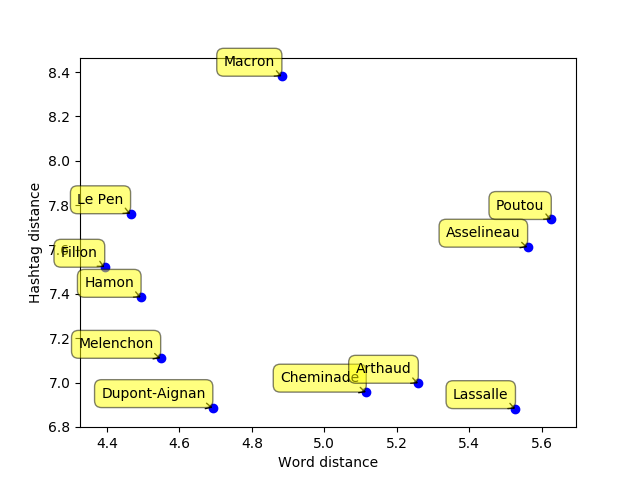
\includegraphics[width=\textwidth]{distances.png}
\caption{Sum of the distance to the other candidates, all words on $x$ and hashtags on $y$}
\end{figure}

It is interresting to see that Emmanuel Macron is the most different in hashtags.

\section{Data Mining}
\subsection{Kmeans and Hierarchical clustering}
We have implemented k-means and Hierarchical clustering.
For two clusters weobtain the same result with both methods.


\begin{figure}
\begin{center}
\begin{multicols}{2}
\label{fig:image3}
\begin{tabular}{ | c | c |}
\hline
Poutou & Melenchon\\
Cheminade & Fillon\\
Arthaud & Hamon\\
Lassalle & Le Pen\\
Asselineau & Macron\\
& Dupont-Aignan\\
\hline
\end{tabular}
\caption{Words Similarities}
\bigskip

\begin{tabular}{ | c | c |}
\hline
Marcon & Melenchon\\
& Fillon\\
& Hamon\\
& Le Pen\\
& Dupont-Aignan\\
& Poutou\\
& Cheminade\\
& Arthaud \\
& Lassalle \\
& Asselineau \\
\hline
\end{tabular}
\bigskip
\caption{Hashtags Similarities}
\end{multicols}
\end{center}
\end{figure}

We can find that for the words there is a repartition minor/leading candidates and that for the hashtags Macron is alone.

\subsection{Variation over time}
We have observed this partition for different periods, since our data cover a few years.

\begin{figure}
\begin{center}
\begin{multicols}{2}
\label{fig:image5}
\begin{tabular}{ | c | c |}
\hline
Melenchon & Fillon\\
Poutou & Le Pen\\
Cheminade & Macron\\
Hamon & Asselineau\\
Arthaud & Dupont-Aignan\\
Lassalle \\
\hline
\end{tabular}
\caption{Before the campaign Hierarchical clustering on hashtags}
\bigskip

\begin{tabular}{ | c | c |}
\hline
Melenchon & Poutou\\
Fillon & Cheminade\\
Hamon & Arthaud\\
Le Pen & Lassalle\\
Macron & Asselineau\\
& Dupont-Aignan\\
\hline
\end{tabular}
\bigskip
\caption{During the campaign Hierarchical clustering on hashtags}
\end{multicols}
\end{center}
\end{figure}

We can see that before the campaign the clustering if rigth/left candidates but during the campaign it is major/minor candidates.


\section{Observations}
The drowback of not using semantic is that there is no link between words with the same meaning, and even between singular and plural words.


\end{document}